\chapter{Soft Brownian Offset}

Soft Brownian Offset (SBO) è un algoritmo per la generazione di dati sintetici fuori dalla distribuzione (Out of Distribution OOD). 

È stato sviluppato da ~\cite{sbo} inizialmente per poter migliorare il rilevamento dei dati fuori dalla distribuzione, si pensi ad esempio nel caso dei cyber-physical systems (CPS) e.g. auto a guida autonoma, dove il rilevamento di eventi fuori dalla distribuzione è di vitale importanza ~\cite{yuhasEmbeddedOutofdistributionDetection2021}.

Per questo scopo i dati generati necessitano di essere non troppo dissimili da quelli originali, perché altrimenti il modello potrebbe soffrire di "overconfidence" ~\cite{amodeiConcreteProblemsAI2016}

SBO si basa sul "Gaussian Hyperspheric Offset" che cerca di creare i dati OOD campionando attraverso una ipersfera attorno ai dati dentro la distribuzione (In Distribution IN).

Partendo da quest'ultimo algoritmo, SBO permette di utilizzare qualsiasi punto del dataset e traslarlo in modo da avere una certa distanza minima dagli altri punti. Dopodichè i punti vengono processati da un autoencoder (AE) addestrato su un particolare dataset. La figura \ref{fig:sbo_schema} mostra graficamente questo approccio. Nel nostro caso, non utilizzeremo una rete neurale bensì XGboost.


\begin{figure}[htpb]
    \centering
    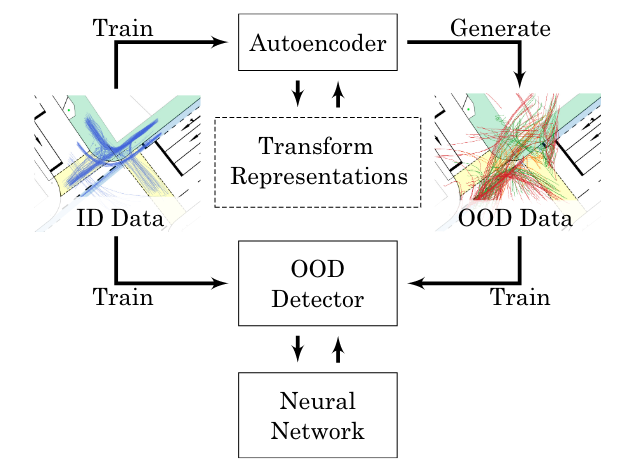
\includegraphics[width=\textwidth,height=10cm,keepaspectratio=true]{img/sbo_schema.png}
    \caption{
        Schema che rappresenta l'approccio utilizzato da SBO. Inizialmente i dati ID vengono usati per addestrare l'autoencoder e successivamente vengono generati i dati OOD tramite SBO. Questi poi vengono decodificati dall'AE per integrarsi nel dataset iniziale. Infine, viene addestrata una rete neurale, nel nostro caso invece, utilizzeremo XGBoost.
    }
    \label{fig:sbo_schema}
\end{figure}

